\chapter[\texttt{eyeris}: Flexible, Extensible, and Reproducible Pupillometry Preprocessing]{\texttt{eyeris}: Flexible, Extensible, and Reproducible Pupillometry Preprocessing in R}\label{ch:eyeris}

The measurement of pupil size and its relation to cognition dates back to the late 1800s with investigation of the pupillary light reflex \parencite{haab1886vortrag}. More than a century later, pupillometry underwent a present-day (re)discovery, establishing pupil size as an integrated psychophysiological readout of cognitive processes such as attention. More specifically, pupillometry offers a non-invasive window into the human mind and brain, and is sensitive to environmental (i.e., luminance, focal distance) and cognitive (i.e., alerting, orienting, attention, executive functioning) changes \parencite{huang2024locus,strauch2024forgotten,strauch2022pupillometry}.

The breadth of cognitive processes that have been associated with pupil size dynamics is expansive, including – but not limited to – emotional arousal \parencite{bradley2008pupil,oliva2018pupil}, mental effort \parencite{kahneman1966pupil,kramer2013processing}, fatigue/task performance \parencite{astonjones2005integrative,eldar2013effects,knapen2016cognitive,mcginley2015cortical,murphy2011pupillometry}, response preparation \parencite{einhauser2008pupil,reimer2014pupil}, uncertainty/decision-making \parencite{gee2014decision,jepma2011pupil,kawaguchi2018differentiating}, prediction error \parencite{alamia2019pupil}, working memory \parencite{keene2022pupillometry,robison2019pupillometry,unsworth2015individual,unsworth2017importance,unsworth2017locus}, and episodic memory \parencite{clewett2020pupil,madore2020memory,madore2022readiness,miller2019individual,miller2020variation,robison2022pupillary,schwartz2025attending}.

As highlighted above, the majority of pupillometry studies use pupil size as an assay of attentional engagement or examine the impact of cognitive processes on pupil size \parencite{kristjansson2009detecting,madore2020memory,vandenbrink2016pupil}. Pupil size is not only linked with various cognitive processes, but also has specific neural substrates, such that pupil diameter dynamics are oftentimes interpreted as a non-invasive (indirect) surrogate of locus coeruleus-noradrenergic (LC–NA) neuromodulatory activity \parencites{he2020age}{joshi2016relationships}[cf.][]{megemont2022pupil}. In humans, pupil diameter has been shown to covary with functional magnetic resonance imaging (fMRI) blood-oxygenation level–dependent (i.e., BOLD) activity in LC \parencite{murphy2014pupil}. More recently, fMRI has been used to identify neural networks in the human brain associated with pupil diameter dynamics in healthy young and older adults and revealed decreases in functional connectivity within a putative pupil diameter network with healthy aging \parencite{wu2025probing}. In most studies, analyses of these pupil data are conducted offline following data collection, although there are also real-time applications providing causal evidence confirming the use of moment-to-moment pupil dynamics as an assay of attentional engagement \parencite{keene2022pupillometry,meissner2024self,schwartz2024real,schwartz2025attending}. Additionally, it is worth noting that given LC’s central role in regulating autonomic function and arousal \parencite{poe2020locus,samuels2008functional} and that LC is the first brain region to develop tau pathology in Alzheimer’s disease \parencite{betts2019locus,braak2011alzheimer,holper2022tau,spires2014intersection}, pupillometry is also being used as a noninvasive window into cognitive aging \parencite{elhaj2024pupillometry,kim2024pupillometry,piquado2010pupillometry}.

Consequently, collecting high-quality pupil data and appropriately analyzing these data are critical for advancing both theories of cognition as well as translational applications of pupillometry. Moreover, data preprocessing is a fundamental prerequisite to high quality pupillometry data analysis \parencite{fink2024from,hershman2024processing,kret2019preprocessing,laeng2024methodological,mathot2023methods,steinhauer2022publication,vanrij2019analyzing}. In pupillometry research, experimenters deal with fewer time series, at most two for binocular recordings, compared to electroencephalography (EEG) or fMRI, but many of the same principles apply: handling missing data, excluding artifacts, and smoothing out physiologically irrelevant noise, to name a few.

Numerous researchers have contributed excellent software packages to the community over the years to aide others in preparing and analyzing pupillometry data without the need to implement core preprocessing functions themselves \parencite[e.g.,][]{forbes2020pupillometryr,geller2020gazer,hershman2019chap,kinley2021pupl,tsukahara2020pupillometry}. However, most of the existing tools only provide rigid preprocessing specifications, often have been factored out of particular analysis projects, and/or do not empower users to be deliberate in preprocessing choices and to compare visualizations of preprocessed pupil data to that of raw pupil data.

Thus, a critical gap in current pupillometry research is the absence of an integrated, standardized, and adaptable preprocessing pipeline – a point emphasized by \textcite{mathot2023methods}, who note:
There is no commonly agreed-upon workflow for conducting cognitive-pupillometry experiments: design criteria, preprocessing steps, and statistical analyses all differ vastly between studies. Some attempts at standardization have been made, but these are not easily applicable to cognitive pupillometry […] Furthermore, guidelines are often conceptual rather than specific implementations, and the lack of concrete examples and code makes it difficult for researchers to incorporate these guidelines into their own workflow. (p. 3055)

In contrast, tools developed for other neuroimaging modalities over the past couple of decades, notably fMRIPrep for fMRI data \parencite{esteban2020analysis,esteban2019fmriprep}, have defined new standards for transparent and reproducible data preprocessing workflows. While widely used software packages such as EEGLAB \parencite{delorme2004eeglab} and MNE-Python \parencite{gramfort2013meg} for M/EEG provide extensive preprocessing functionality, they operate primarily as flexible toolboxes, leaving decisions about preprocessing steps, their order, and parameter settings to individual researchers. More recently, efforts to build standardized preprocessing pipelines on top of these toolboxes – such as PREP \parencite{bigdelyshamlo2015prep} and Automagic \parencite{pedroni2019automagic} for EEG, or MNE-BIDS-Pipeline (\url{https://mne.tools/mne-bids-pipeline/stable/}) for M/EEG – reflect a growing recognition of the need for more prescribed, reproducible preprocessing workflows.

However, developing and sustaining robust preprocessing pipelines is not trivial. Many scientists with strong domain expertise lack formal training in computer science or software engineering \parencite{chen2025exploring,segal2008scientists}, a likely contributing factor to the inadvertent adoption of common programming ``anti-patterns'' when writing analytic code \parencite{wilson2014best}. In fact, nonreproducibility in science often results from some combination of poor programming practices \parencite{hatton1997texperiments,hatton1994accurate,merali2010error,miller2006scientists}, suboptimal and inattentive code and data management and sharing practices \parencite{frank2025replication,gorgolewski2016practical,kovacs2024opening}, and/or insufficient transparency about the specific details underlying each step taken in between to transform raw data into a high quality format appropriate for inferential statistics \parencite{poldrack2019computational}. Over and above these pitfalls is the ``garden of forking paths'' problem and the culprit of Type I (i.e., false positive) errors in extant literature \parencite{gelman2013garden,poldrack2017scanning,simmons2011false}.

In the context of psychological science, flexibility in data analysis and reporting has been implicated as a prominent contributor to the replication and reproducibility crisis \parencite{hardwicke2021analytic,hardwicke2018data,hardwicke2022estimating,ioannidis2005why,osc2015estimating}. Likewise, the garden of forking paths for psychophysiological data is a slippery slope: when researchers are afforded more preprocessing pathways and analytic degrees of freedom, even small adjustments to the way data are preprocessed (e.g., digital filter design, handling of missing data, artifact removal) can impact the outcomes and interpretations a researcher may draw from their data \parencite{soskic2024garden}.

To fill this gap in robust preprocessing pipelines for pupillometry data, we developed eyeris, an R package dedicated to providing unified standards for pupillometry preprocessing \parencite{schwartz2025eyeris}. With eyeris, we not only intend to provide users with an extensible toolkit for conducting robust pupillometry preprocessing, but critically aim to contribute to standardizing best practices in pupillometry research (especially for cognitive pupillometry; see \textcite{mathot2018pupillometry} for a review discussing pupil responses, the neural pathways subserving these pupillary responses, and their relationship to high-level cognition). We should note that we are not the first group to put forth a recommended set of preprocessing guidelines for cognitive pupillometry. Here, we have built upon the comprehensive guide to cognitive pupillometry preprocessing put forth by \textcite{mathot2023methods}; their stated aim is to provide ``guidelines [that] are meant to be illustrative, rather than prescriptive; that is, we show how things could be done – rather than how they should be done – in order to implement a workflow that is both easy to implement and that meets contemporary standards for good scientific practice'' (p. 3056). In contrast, we adopt a prescriptive, rather than merely illustrative, approach to pupillometry preprocessing workflows.

Here, we argue that a standardized cognitive pupillometry preprocessing workflow is essential to limit the number of forking paths available to researchers during analysis. In other words, without consistent preprocessing, studies leveraging pupillometry to advance key theories in psychological science could be hindered by high degrees of freedom and vulnerable to unintended mistakes during preprocessing. As such, our accompanying R package is designed with ``glass box'' principles \parencite[see][]{esteban2019fmriprep,poldrack2019computational}, thereby equipping both novice and experienced pupillometry researchers with key tools needed to appropriately transform raw pupillometry data into a format well-suited for downstream analysis, visualization, and statistical inference. Embracing a carefully designed pipeline is highly beneficial, as it enables researchers to focus on hypothesis testing with minimal worry about whether the data were preprocessed correctly. In this era of open-source software, it is also important to allow experienced users to inspect and modify steps in a preprocessing pipeline with minimal hurdles.

eyeris strongly encourages users to follow a prescribed set of steps in a particular order and with carefully selected default parameters. The overarching aim is to avoid unnecessary preprocessing decisions that may lead to issues when made with incomplete knowledge of some of the nuances of signal processing. At the same time, eyeris provides transparent access and configurability to all preprocessing steps in a user-friendly fashion, which is supported by its modular, glass-box design (Figure~\ref{fig:eyeris-fig1}, Box~\ref{box:glassbox-example}). This design approach greatly reduces the burden of usage by removing the need to develop lengthy scripts for individual use cases \parencite{varoquaux2016beyond}.

\begin{eyerisbox}{glassbox-example}{Example usage of the \texttt{glassbox()} pipeline wrapper}
\begin{lstlisting}
library(eyeris)

path_to_demo_dataset <- eyelink_asc_demo_dataset()

cleandata <- glassbox(file = path_to_demo_dataset)
#> [ OK ] - Running eyeris::load_asc()
#> [ OK ] - Running eyeris::deblink()
#> [ OK ] - Running eyeris::detransient()
#> [ OK ] - Running eyeris::interpolate()
#> [ OK ] - Running eyeris::lpfilt()
#> [SKIP] - Skipping eyeris::detrend()
#> [ OK ] - Running eyeris::zscore()

plot(cleandata)
#> ! Plotting block 1 from possible blocks: 1
\end{lstlisting}
\end{eyerisbox}

\begin{figure}[!tbp]
	\centering
	\includegraphics[width=1\linewidth]{figures/eyeris-fig1.jpg}
	\caption[A sample workflow for the eyeris R package]{A sample workflow for the eyeris R package. The example code shows an end-to-end preprocessing pipeline, starting at raw data from the tracker to epoched and derived files ready for visualization and analysis. Here, we draw particular attention to the flexibility eyeris offers for segmenting (i.e., epoching) trials from the continuous pupil time series. In this demonstration, the \texttt{epoch()} function will find all event messages from the recording session that include the ``\texttt{PROBE\_START\_*}'' wildcard expression and extract 1-second prior to as well as 1-second following the onset timestamp from the matched message string (and will name the resulting tidy data frame of extracted pupil epochs: ``prePostProbe'', which will be saved to the resulting eyeris S3 class ``list'' object — not shown here). Note, the ``\texttt{\{trial\}}'' syntax is a feature that enables a user to tell eyeris to not only treat that portion of the string as a wildcard expression, but also to take whatever substring matched to that position of the string and place its content in a new column with the header title: trial. This feature was designed with the intention to streamline the extraction of metadata embedded within tracker event messages into the same tidy data frame as any corresponding pupil data extracted from these events. The \texttt{epoch()} function is quite flexible and can handle a wide range of event message-string configurations; an in depth walkthrough can be found in the package documentation. Created in BioRender \parencite{schwartz2025eyerispkg}. \url{https://BioRender.com/vkahl3u}.}
	\label{fig:eyeris-fig1}
\end{figure}
\FloatBarrier

\section{Method}
\subsection{eyeris R package}
The eyeris R package is actively maintained and available on both CRAN and GitHub (see Code Availability). Box~\ref{box:installation} describes the three recommended methods for installing eyeris.

\begin{eyerisbox}{installation}{\texttt{eyeris} R package installation options}
\begin{lstlisting}
# (a) to install the latest stable release from CRAN:
install.packages("eyeris")

# (b) using Posit's pak approach to install packages interactively:
# install.packages("pak")
pak::pak("eyeris")

# (c) to install the bleeding edge development version:
# install.packages("devtools")
devtools::install_github("shawntz/eyeris")
\end{lstlisting}
\end{eyerisbox}

\subsection{Entry-point function: glassbox()}
The primary entry point for preprocessing pupillometry data in eyeris is the glassbox() function, which offers an opinionated, fully transparent preprocessing pipeline. This “glass-box” design contrasts with “black-box” workflows by allowing (and encouraging) users to understand and evaluate the consequences of each processing step on their data. Within eyeris, the glassbox() function completely streamlines the preprocessing workflow, enabling researchers to seamlessly transform raw pupil data into a high-quality, standardized format ready for analysis and visualization.

We designed glassbox() to operate in both interactive and headless modes. In the interactive mode, users are well-positioned to evaluate pre- and post-processing plots of their pupil time series data following the execution of each pipeline step, with prompts to continue or modify parameters as needed. In the headless mode, users are permitted to automate preprocessing of pupil datasets of any size, including large-scale pupillometry datasets on cloud computing clusters, using recommended default parameters without manual intervention.

Users are permitted to override the default parameters of any preprocessing step within glassbox() by passing a named list of arguments to the specific function (e.g., deblink = list(extend = 100)) as arguments to the glassbox() function. Taken together, eyeris’ flexibility out-of-the-box facilitates real-time parameter optimization and empowers researchers to tailor the pipeline to their specific data characteristics and research questions in a transparent fashion.

\subsection{Sequential preprocessing steps of the glass-box pipeline implementation and usage}
The glassbox() pipeline executes a fully transparent prescribed sequence of pupillometry preprocessing steps, which are also available as individual modular functions (see Box~\ref{box:glassbox-example}). Although users are able to build their own pipelines using the individual modules, we strongly recommend that users invoke the glassbox() pipeline function, given each step is critical and must be performed in a specific order to avoid unexpected data modifications that could compromise downstream analyses. Below, we demonstrate the sequence of core methods that comprise the glassbox() function to showcase both its flexibility and its syntactic simplicity.

\subsection{Loading and parsing data: eyeris::load\_asc()}
This initial step builds upon the eyelinker::read.asc() function and parses SR Research EyeLink .asc files, extracting raw time series data, event messages, blink events, and various metadata from the file header. The load\_asc() function within eyeris also supports automatic handling of multiple recording segments (i.e., blocks) within a single .asc file and offers options for gracefully handling binocular data out-of-the-box (e.g., averaging left and right eye pupil sizes, or processing them independently). Note, it is critical that users load their data using eyeris::load\_asc() given there are a number of configuration steps eyeris performs to ensure data can be seamlessly passed through each pipeline module.

\subsection{Blink artifact removal: eyeris::deblink()}
The deblink() function removes blink-related artifacts by NA-padding missing-data periods and their surrounding samples in the pupil time series. Each period of missing data is extended both backward and forward in time by a user-configurable duration (defaulting to 50 ms) to mask the partial-occlusion artifacts that typically flank eye blinks. The extend parameter accepts either a single value for symmetric padding or a two-element vector for asymmetric padding (e.g., c(backward, forward)). The appropriate extend duration may vary across experimental setups or participant populations and can be optimized upon inspection of the diagnostic reports generated by eyeris.

\subsection{Transient artifact removal: eyeris::detransient()}
The detransient() function identifies and removes non-physiological pupil samples – such as transient spikes caused by unstable tracking or head movements – by applying a speed-based threshold. The function computes an approximate pupil change velocity using finite differences and flags samples whose speed exceeds a threshold derived from the Median Absolute Deviation \parencite[MAD;][]{arachchige2024confidence,hampel1968contributions,hampel1974influence,leys2013detecting,rousseeuw1993alternatives,rousseeuw1986robust} of the velocity distribution. Specifically, the threshold is defined as the median speed plus n times the MAD value, where the constant n defaults to 16 \parencite{tsukahara2020pupillometry}. For edge cases where the computed MAD or median speed is very small, users may supply a manual threshold via the mad\_thresh parameter to adjust sensitivity.

\subsection{Linear interpolation: eyeris::interpolate()}
The interpolate() function fills in missing pupil samples resulting from the preceding blink removal and artifact detection steps, recovering a contiguous time trace. It applies linear interpolation via the na.approx() function from the zoo package \parencite{zeileis2005zoo}, with edge NAs replaced by the nearest available values. Linear interpolation is well-suited to pupillometry given the relatively slow dynamics of pupil size fluctuations; however, users are strongly encouraged to set cutoff thresholds to exclude trials or periods in which a substantial proportion (e.g., 50\%) of raw data are missing.

\subsection{Low-pass filtering: eyeris::lpfilt()}
The lpfilt() function smooths the pupil time series by applying a low-pass Butterworth filter, with the default passband cutoff at 4 Hz and stopband at 8 Hz. The filter order is automatically determined by the buttord() function from the gsignal package \parencite{vanboxtel2021gsignal} to satisfy the specified passband/stopband frequencies and ripple/attenuation constraints. The resulting filter uses a second-order sections representation for numerical stability. Users may modify the filter design parameters (wp, ws, rp, rs) and inspect the frequency response by setting plot\_freqz = TRUE.

\subsection{Downsampling: eyeris::downsample()}
The downsample() function reduces the sampling frequency of the pupil time series to a user-specified target rate (target\_fs) while preserving the original temporal dynamics of the signal. Unlike binning, downsampling retains individual data points after first applying an automatically designed anti-aliasing low-pass filter to prevent spectral aliasing. As a safeguard, the function raises an error if the resulting passband frequency would fall below 4 Hz, protecting frequency content relevant to pupillary responses. Users can optionally visualize the anti-aliasing filter’s frequency response by setting plot\_freqz = TRUE.

\subsection{Binning: eyeris::bin()}
The bin() function provides an alternative approach to reducing temporal resolution by dividing the time series into equal-duration intervals and computing a summary statistic – either the mean (default) or median – within each bin. The number of bins per second is controlled by the bins\_per\_second parameter, and the resulting timepoints are centered within each interval. Although binning is commonly used in pupillometry research, users should be aware that averaging within bins can attenuate rapid pupillary dynamics; the choice between downsampling and binning should therefore be guided by the specific research question.

\subsection{Detrending: eyeris::detrend()}
The detrend() function removes slow linear drifts from the pupil time series by fitting a linear model of pupil size as a function of time and returning the residuals. This step can be useful for removing gradual drifts such as the commonly reported “time-on-task effect”, but is disabled by default in eyeris for two reasons: first, trial-level baseline correction often renders detrending unnecessary \parencite[see][for a detailed discussion of the tradeoffs between subtractive and divisive baseline correction approaches]{mathot2018safe}, and second, linear detrending is an imperfect correction – slow trends in pupil size are often nonlinear, and applying a linear detrend can introduce new biases to the signal (Strauch et al., 2015). Moreover, slow trends may reflect physiologically meaningful tonic arousal levels that should be preserved depending on the research question (see Section~\ref{sec:preproc-steps} for a more detailed discussion). Users may enable this step within glassbox() by setting detrend = TRUE when the removal of slow linear trends is appropriate for their research question.

\subsection{Z-scoring: eyeris::zscore()}
The zscore() function normalizes the pupil time series to have a mean of 0 and a standard deviation of 1 by mean-centering and scaling, analogous to base::scale(). This normalization facilitates trial-level and between-subjects analyses, as the arbitrary units of pupil size do not scale consistently across participants or recording sessions. Because eyeris is designed to preprocess one block of data per participant at a time, each block is z-scored independently; when preprocessed data are later merged, all blocks will have been separately scaled. Z-scoring is enabled by default and can be disabled by setting zscore = FALSE within glassbox().

\section{Additional functions for epoching, exporting, and visualizing pupil data}
In addition to the core preprocessing steps described above, eyeris provides built-in methods to conveniently extract tidy trial-based epochs with optional baseline correction, export BIDS-style derivatives and diagnostic HTML reports, and interactively browse diagnostic plots for tens of thousands of trials at each preprocessing step.

\subsection{Epoching and baseline correction: eyeris::epoch()}
The epoch() function is intended to be used as the final preprocessing step. It creates data epochs of either fixed or dynamic durations with respect to user-supplied event message strings and time limits, and includes an intuitive metadata parsing feature where additional trial data embedded within event messages can be automatically identified and joined into the resulting epoched data frames. The function supports three main event-modes: (i) a single string representing the event message to center epoch extraction around, using specified limits (or, if no limits are provided, extracting data between each subsequent occurrence of the same event); (ii) a vector containing both start and end event message strings, where limits are ignored and the duration of each trial epoch is determined by the number of samples between each matched start–end pair; and (iii) a list of two data frames that manually specify start/end event timestamp–message pairs for extraction from the raw time series, with explicit block number specification.

For event-modes (i) and (ii), the event message string must conform to a standardized protocol so that eyeris knows how to find events and optionally parse included metadata. Users have two primary choices: (a) specify a string followed by a * wildcard expression (e.g., PROBE\_START\*), which matches any messages beginning with that prefix; or (b) specify a string using the eyeris curly-brace syntax (e.g., PROBE\_\{type\}\_\{trial\}), which matches messages following that structure and automatically generates additional metadata columns (e.g., type and trial) in the tidy output. The function also supports optional baseline correction via the calc\_baseline and apply\_baseline parameters, with both subtractive and divisive correction types and flexible specification of the baseline period through either fixed time windows or event-delimited intervals (see Box~\ref{box:epoch} for additional details).

\begin{eyerisbox}{epoch}{Tips \& Tricks: Extracting pupil data from trial epochs with varying durations}
Users may also be interested in extracting the pupil time series for each stimulus/probe from start-to-finish. To illustrate, if each probe was displayed for a variable duration --- perhaps because the participant's response designates the end of that trial --- then the user cannot rely on a fixed-duration epoch extraction method. To demonstrate the power and flexibility of our implementation for this case in \texttt{eyeris}, take, for instance, an expansion of the researcher's event message tags for the probe onsets we discussed in the main text above and suppose that the researcher also included event message tags to signal the end of any given epoch, such as: \texttt{PROBE\_END\_32\_PIANO}. With \texttt{eyeris}, the user can specify their starting boundary to be \texttt{PROBE\_START\_\{trial\}\_\{stimulus\}} and ending boundary to be \texttt{PROBE\_END\_\{trial\}\_\{stimulus\}}, which tells \texttt{eyeris} to grab all samples between each of these boundaries, and additionally, to create new metadata columns in the tidy output data frame containing the third and fourth extracted values in between the underscore separator with column names of \texttt{trial} and \texttt{stimulus}, respectively. See Function: \texttt{epoch()} for additional details.
\end{eyerisbox}

\subsection{Exporting BIDS-like derivatives: eyeris::bidsify()}
The bidsify() function provides a structured way to save preprocessed pupil data in a BIDS-like directory structure. It exports epoched data as well as the raw pupil time series, and formats directory and file name structures based on user-supplied metadata (participant ID, session number, task name, and run number). For multi-block recordings contained within a single .asc file, blocks are automatically numbered as separate runs. The function also supports merging epochs into a single output file, merging runs across blocks, and optionally generating interactive HTML diagnostic reports. These reports include epoch-by-epoch diagnostic plots that can be grouped by a user-specified column variable (defaulting to the matched event label). In the future, we intend for this function to save data in an official BIDS format for eye tracking data (see the proposal currently under review); however, at this time, the function takes a BIDS-inspired approach to organizing output files (see Box~\ref{box:bids}).

\begin{eyerisbox}{bids}{BIDS-like derivatives data structure}
\begin{verbatim}
eyeris/
|- derivatives/
   |- sub-001/
      |- eye/
      |  |- sub-001_task-ret_run-01_desc-timeseries_pupil.csv
      |  |- sub-001_task-ret_run-01_epoch-probe_desc-preproc_pupil.csv
      |- source/
      |  |- figures/
      |     |- run-01/
      |        |- epoch_probe/
      |        |  |- run-01_PROBE_22_1.png
      |        |  |- run-01_PROBE_22_2.png
      |        |  |- run-01_PROBE_22_3.png
      |        |  |- ...
      |        |- run-01_fig-1_desc-histogram.jpg
      |        |- run-01_fig-1_desc-timeseries.jpg
      |- sub-001_epoch-probe_run-01.html
      |- sub-001.html
\end{verbatim}
\end{eyerisbox}

\subsection{Diagnostic visualization: eyeris::plot()}
The plot() function is an S3 plotting method for objects of class eyeris. It plots a single-panel time series for a subset of the pupil data at each preprocessing step, providing a simple method for qualitatively assessing the consequences of the preprocessing recipe and its parameters on the raw pupillary signal. Users can control which preprocessing steps to visualize (defaulting to all), the number and duration of random preview epochs, and whether to display accompanying histograms of pupil samples at each step via the plot\_distributions parameter. A fixed random seed can be set to ensure the same preview epochs are displayed across repeated calls, which is especially useful when iteratively adjusting parameters within and across workflow steps. For multi-block recordings, the block parameter specifies which block to plot.

\subsection{Database storage and analysis}
In addition to the BIDS-like file exports described further in Section~\ref{sec:visual-reports}, eyeris provides an integrated database storage backend for centralized management of preprocessed pupillometry data. Database storage is activated by setting db\_enabled = TRUE within the bidsify() function, which creates or connects to a DuckDB \parencite{raasveldt2019duckdb} database file (.eyerisdb) in the derivatives directory. All data types generated by the preprocessing pipeline – including time series, events, blinks, epochs, epoch summaries, and confounds – are automatically written to the database alongside any CSV exports. For large-scale deployments where storage efficiency and I/O performance are priorities, CSV output can be disabled entirely by setting csv\_enabled = FALSE.

The eyeris database API provides a suite of functions for connecting to, querying, and extracting data from the database without requiring SQL expertise. The eyeris\_db\_summary() function provides a quick overview of the database contents, including available subjects, sessions, tasks, and row counts per data type. The eyeris\_db\_collect() function serves as the primary extraction interface, enabling researchers to aggregate data across multiple subjects in a single call with flexible filtering by subject, session, task, epoch label, and eye. For advanced use cases, direct SQL queries can be executed through the underlying DBI connection obtained via eyeris\_db\_connect().

To support data sharing and distribution of large databases, eyeris includes chunked export functionality. The eyeris\_db\_to\_chunked\_files() function processes data incrementally (defaulting to 1 million rows per chunk) and writes the output to CSV or Parquet files, automatically splitting files that exceed a configurable size threshold (defaulting to 50 MB). For formal data distribution, eyeris\_db\_split\_for\_sharing() partitions the database into portable chunks that can be reconstructed by collaborators using eyeris\_db\_reconstruct\_from\_chunks(). The Parquet format is also supported, offering 50–80\% file size reduction compared to CSV, faster read performance, and preserved numeric precision.

\section{Results}
\subsection{Key Features \& Innovations}
Here, we introduce eyeris with the goal of making pupillometry preprocessing more efficient, reproducible, and conducive for reliable inferences as well as providing researchers greater confidence when analyzing their pupillometry data.

\subsubsection{Common pupillometry preprocessing steps performed in a prescribed order.}\label{sec:preproc-steps}
Pupillometry time series require a relatively small number of preprocessing steps compared to multivariate data (such as EEG and fMRI); yet, there is a more defined set of issues to be addressed when preprocessing pupil size data. Critically, these preprocessing steps must be completed in a certain order to avoid unexpected modifications of the data in a way that could compromise downstream analyses. In this section, we describe some of the most common preprocessing steps for pupillometry data, which are implemented in the current version of eyeris. While additional steps might be added in the future, some of the basic principles covered here will be applicable in general.

First, preprocessing of pupil sizes needs to handle artifactual or missing data due to eye blinking, movement, or simply incorrect pupil detection and measurement by the eye tracker. Most existing commercial eye trackers, including SR Research EyeLink, have built-in blink detection methods that will annotate blink periods in exported data. One can easily recognize blink periods when the pupil size becomes 0/NaN for a brief period of time. However, it is important to recognize that there are often blink-related artifactual changes in pupil size surrounding an eye blink, which can be due to the eyelid rapidly covering the pupil area detected by the camera, resulting in rapidly diminishing pupil size before becoming zero. In contrast, as the eyelid opens, there is a brief period of rapidly increasing pupil size when the camera detects a partial pupil. Occasionally, eye trackers may incorrectly lock onto other structures in the camera’s field of view, such as eyebrows and glasses frames, as they may become more probable pupil targets compared to partially occluded pupils during blinking. This can also result in fluctuations in recorded pupil sizes. As such, eyeris removes blink periods using the deblink() function with an extend duration (defaults to 50 ms) bleeding both backward and forward in time to mask neighboring time periods that may contain such artifacts. Note, the extend duration parameter may need to be adjusted for different experimental setups, certain groups of participants, or even for individual participants, which can be determined on a case-by-case basis upon inspection of visual diagnostic reports.

While commercial eye trackers can mark blink periods for easy exclusion, there are also artifactual pupil size measures that could occur in recordings due to unstable pupil tracking or eye/head movements. These non-blink disruptions of pupillometry measurement often result in transient and abrupt changes in recorded pupil sizes, commonly visible as spikes in the time series. eyeris detects and removes such transient artifacts using the detransient() function. Under the hood, detransient() computes an approximate pupil change velocity by taking the first-order difference divided by sampling interval and detects outliers using the MAD procedure \parencite{arachchige2024confidence,hampel1968contributions,hampel1974influence,leys2013detecting,rousseeuw1993alternatives,rousseeuw1986robust}. In our experience, most artifacts in pupillometry data can be captured using the simple detransient() method, thereby excluding non-physiological measures. However, noisier recordings with different eye tracker hardware may require more elaborate artifact detection algorithms, such as to remove sustained periods of outlying pupil sizes instead of velocity. Users are strongly encouraged to expand on the function given their data and contribute to eyeris with additional methods to remove artifact periods (see Box~\ref{box:extensions} and Appendix~\ref{app:custom-extensions} for more information about extensibility and developing custom extensions in eyeris).


Once data from blink and artifact periods are removed, the next step in pupillometry preprocessing is to interpolate over these periods to recover a contiguous time trace of pupil sizes \parencite{mathot2013simple}. While not strictly required for certain types of pupillometry analysis – such as averaging across trial periods for a univariate measure – many recent analytic approaches for pupillometry data leverage each sampled time point to uncover temporal dynamics in changes of pupil sizes \parencite{clewett2020pupil,johansson2018pupil,steinhauer2004sympathetic,urai2017pupil,vanslooten2018how,verney2004pupillary,widmann2018emotion}. With these forms of analysis, avoiding missing data in certain periods provides more evenly distributed statistical power across time points (even with ”guessing” of missing data through interpolation). Accordingly, eyeris uses the interpolate() function and takes the simplest approach of linear interpolation due to the relatively slow nature of pupil size fluctuations. However, users are strongly encouraged to adopt cutoff thresholds to exclude periods or trials when more than a certain percentage (such as 50\%) of raw data is missing.

It is evident that the interpolation steps should occur after missing-data detection, but it is less clear if, when, and how smoothing of typically noisy pupillometry data should take place. Smoothing of pupil sizes over time is commonly employed in the literature \parencite{steinhauer2022publication} both to provide cleaner time trace visualizations and to reduce sporadic temporal dynamics that may be unrelated to underlying neurocognitive processes of interest. Smoothing is justified for pupil sizes with relatively slow dynamics but should always occur after blink and artifact detection to avoid contaminating neighboring samples during smoothing. In addition, smoothing can be achieved in multiple different ways, such as with moving averages or low-pass filtering. eyeris uses the lpfilt() function to apply a low-pass Butterworth filter with passband starting at 4 Hz and stopband starting at 8 Hz. Note, the lpfilt() function here uses a minimum-order Butterworth filter, whose order is obtained with the buttord() function from the gsignal package \parencite{vanboxtel2021gsignal} to meet the defined passband and stopband cutoff frequencies (i.e., wp, ws) and ripple/attenuation requirements (i.e., rp, rs). The filter created by the gsignal::butter() function is returned in the second-order sections format. Users can easily modify the filter design parameters to achieve different smoothing results, but should always inspect the frequency response of the filter to ensure sufficient signal attenuation at higher frequencies and minimal ripples in the passband. The frequency response can be visualized by passing the plot\_freqz = TRUE parameter to lpfilt().

Pupil sizes can fluctuate at a slow pace over the course of an entire recording; for example, the commonly reported decreasing trend during a cognitive task \parencite[a.k.a., the ``time-on-task effect'';][]{beatty1982phasic,hopstaken2015multifaceted,martin2022pupillometry,massar2016rewards,steinhauer2022publication,unsworth2016pupillary,zhao2019pupillometry}. Depending on the scientific questions at hand, removal of this time-on-task effect may be desirable. eyeris provides the detrend() function to remove a linear trend over the entire recording. However, it should be noted that pupillometry analysis often employs baseline correction in a trial-by-trial design; as such, detrending might be unnecessary and could also increase the risk of introducing artifacts in the data if an extreme trend gets extracted (although unlikely as these artifacts were likely removed in the preceding steps). Moreover, high-pass filtering is discouraged as a way to remove slow trends in pupillometry data because designing a filter with a sufficiently sharp cutoff at the lower frequency end is difficult; failing to implement a proper filter design could drastically change the waveforms of pupil sizes that contain frequency content at approximately 1 Hz. Lastly, slow trends in pupil sizes might be physiologically meaningful, as tonic pupil sizes may reflect tonic arousal levels \parencite{astonjones2005integrative,groot2021probing,joshi2020pupil,madore2020memory,madore2022readiness,murphy2011pupillometry,schwartz2025attending,smallwood2012insulation,tsukahara2016relationship,unsworth2018tracking}. Depending on the target research question(s), such trends may need to be preserved for downstream analysis. Therefore, eyeris defaults to not performing detrending during preprocessing.

Finally, there has been an ongoing debate regarding z-scoring normalization of pupillometry data. Some have argued against doing so outside of MRI contexts \parencite{steinhauer2022publication}. Normalizing pupil sizes by the mean and variance can introduce additional challenges in interpreting derived measures. Yet, it can also be argued that in the absence of normalization, pupil data across individuals cannot be easily pooled together for statistical inference, even if the non-normalized pupil sizes faithfully reflect individuals’ physiological responses. To illustrate, older adults and young adults may have differences in physical constraints that impact how much the pupil can dilate during cognitive performance. Not accounting for such differences may lead to the conclusion that older adults have weaker pupillary responses to certain stimuli (such as a loud tone). However, if different ranges of pupil fluctuations across individuals are accounted for by using z-scored pupil sizes, older adults may show comparable responses to such stimuli relative to their normal ranges of pupillary responses \parencite{he2020age}. Therefore, while older adults may show attenuated changes in pupil size due to physiological changes in muscles controlling pupil dilation, their cognitive arousal response to tone stimuli may not be preferentially reduced to suggest a selective deficit. Similar examples can be found even within a homogeneous group, since differences across individuals and across blocks/sessions are often present in each recording \parencite[e.g.,][]{madore2020memory}. Averaging non-normalized pupillary responses produces a metric biased by absolute pupil size, potentially confounding the cognitive (pupil) signal of interest with physiological variability.

Hence, z-scoring pupillometry data allows one to focus on the relative dynamics of fluctuations in pupil sizes rather than the first-level characteristics such as mean pupil sizes or absolute changes. It should be emphasized that z-scoring automatically makes the assumption that the variances accountable by changes in the absolute value or range of pupil sizes are irrelevant to target scientific questions. In many modern applications of pupillometry within psychological sciences, this is not an unreasonable assumption \parencite[i.e.,][]{bradshaw1969background,gilzenrat2010pupil,he2020age,peysakhovich2017impact,vangerven2004memory}. Therefore, eyeris defaults to perform z-scoring normalization with the zscore() function. One can easily turn off z-scoring during preprocessing, and we strongly encourage users to carefully consider how the decision to apply or forgo normalization of pupil sizes will impact downstream interpretations of their data, particularly when absolute pupil size or cross-session and cross-individual differences are relevant to the scientific question at hand.

\subsubsection{A modular signal processing workflow with carefully chosen parameters ensures efficient and robust pupillometry preprocessing.}

One key strength of the eyeris framework is its modularity. Each preprocessing function within eyeris is a wrapper around a core pipeline operation that automatically tracks, versions, and stores preprocessing states for any pupillometry dataset being processed in eyeris. This enables a ”plug-and-play” experience when using eyeris: users have the option to use our recommended glassbox() method, as well as the ability to construct novel extensions and custom pipelines. Critically, this modular architecture promotes both adaptability and extensibility, facilitating the streamlined integration of custom preprocessing methods directly into the default workflow (Boxes~\ref{box:glassbox-example},\ref{box:quickstart},\ref{box:custom-params},\ref{box:extensions}; Appendix~\ref{app:custom-extensions}).

\begin{eyerisbox}{quickstart}{Tips \& Tricks: Consider preprocessing your data with \texttt{eyeris::glassbox()} rather than manually calling individual steps}
Although we encourage most users to use the \texttt{glassbox()} function for simplicity and adherence to signal processing best practices, advanced users can create custom preprocessing steps that seamlessly integrate into the workflow (and thus will behave like native package functions without the need for hacky integrations). Therefore, it is imperative that the custom pipeline steps conform to the \texttt{eyeris} protocol to ensure maximum compatibility and reproducibility with downstream functions. We provide a thorough vignette that walks users through the process of creating custom extensions in the package documentation (\url{https://eyeris.shawnschwartz.com/articles/custom-extensions.html}) and in Section~\ref{sec:dev-features}.
\end{eyerisbox}

We recommend that users start with the glassbox() function to reduce the probability of inadvertently introducing sub-optimal computations or errors that could arise when reimplementing the individual steps underlying the preprocessing pipeline – both within and between projects. The glassbox() function allows users to make flexible adjustments – such as disabling a particular step and/or changing the default settings for a step – by passing in parameter arguments (see Box~\ref{box:custom-params}). A strength of the built-in glassbox() function compared to the many extant pupillometry packages is the framework it provides for rapidly preprocessing pupillometry data without requiring users to rely on copy-pasting complex step-by-step functions employed on a toy dataset from a vignette (which may not necessarily be optimized for the variety of forms that real-world pupillometry data come in). Furthermore, even when the instructions and functions supplied in a vignette of a package work ”out-of-the-box” after pasting them into a custom script, it is still the user’s responsibility to ensure that every step was not only run, but done so in the correct order (with respect to the best practices of signal processing). Failing to do so could lead to unexpected and possibly detrimental results for the conclusions researchers will ultimately draw from the data. Therefore, we aim to facilitate this process to enable users to more easily engage with preprocessing steps by using a package, rather than moving away from them. With the eyeris glassbox() function, users can take a pupillometry recording file directly from a participant session, and in a short amount of time can go from raw to fully preprocessed data with detailed diagnostics for quality control in approximately three lines of code (Box~\ref{box:glassbox-example},\ref{box:quickstart}; Figure~\ref{fig:eyeris-fig2}).

\begin{eyerisbox}{custom-params}{Overriding default parameters in the \texttt{eyeris::glassbox()}}
\begin{lstlisting}
output <- glassbox(
  rawdata,
  confirm = FALSE,
  deblink = list(extend = 40),
  detransient = FALSE,
  lpfilt = list(plot_freqz = FALSE)
)
#> [ OK ] - Running eyeris::load_asc()
#> [ OK ] - Running eyeris::deblink()
#> [SKIP] - Skipping eyeris::detransient()
#> [ OK ] - Running eyeris::interpolate()
#> [ OK ] - Running eyeris::lpfilt()
#> [SKIP] - Skipping eyeris::detrend()
#> [ OK ] - Running eyeris::zscore()
\end{lstlisting}
\end{eyerisbox}

However, one critique of encapsulating a series of preprocessing steps into a single wrapper function – like glassbox() – is the regression towards a more black-box-like implementation. eyeris circumvents this pitfall in two key ways. First, the glassbox() function has two modes: interactive and headless. The interactive mode allows users to evaluate the consequences of the parameters used within each step on their data in real time, thereby facilitating an easy-to-use workflow for parameter optimization on any given dataset. In essence, this interactive process takes each recommended step and forces the user to evaluate both pre- and post-processing plots of time series for all steps in the default pipeline, with interjecting prompts to continue or modify parameters before moving forward. This stepwise approach to optimizing signal preprocessing parameters that yield satisfactorily de-noised pupil time series data reduces the opacity of the wrapper function to a transparent and engaging experience. The headless mode permits users to run the pipeline as-is on a dataset of any size – be it on their computer locally or on a cloud computing cluster – to preprocess large-scale pupillometry datasets using our recommended default parameters without manual intervention.

\begin{eyerisbox}{extensions}{Deconstructing \texttt{glassbox()}: Using the flexible \texttt{eyeris} primitives}
\begin{lstlisting}
system.file("extdata", "memory.asc", package = "eyeris") |>
  load_asc(block = "auto") |>
  deblink(extend = 50) |>
  detransient(n = 16) |>
  interpolate() |>
  lpfilt(wp = 4, ws = 8, rp = 1, rs = 35, plot_freqz = TRUE) |>
  # eyeris::detrend() |> # optional (read docs before enabling)
  zscore()
\end{lstlisting}
\end{eyerisbox}

Second, eyeris stores the history of preprocessing steps and parameters for every action made on a raw dataset so that any derived data from the pipeline can be easily reproduced without additional steps needed from the researcher. Specifically, all of these data are saved to interactive HTML files (Figure~\ref{fig:eyeris-fig2}), which contain numerous diagnostic plots for every step of the pipeline, automatically parsed tracker metadata, and a snapshot of the actions performed at each step of the workflow (see Section~\ref{sec:visual-reports}). Thus, using eyeris to deploy a large-scale preprocessing workflow on a headless computing architecture allows researchers to manually scrub their data sets for each run from every subject at every step of preprocessing without additional custom scripting. Critically, these interactive reports provided by eyeris go above and beyond within-study data quality control by automatically capturing and recording data and signal processing provenance in a standardized schema \parencite{mackenziegraham2008provenance} – an essential feature for analytic reproducibility, lacking in many existing pupillometry preprocessing tools.

\begin{figure}[!tbp]
	\centering
	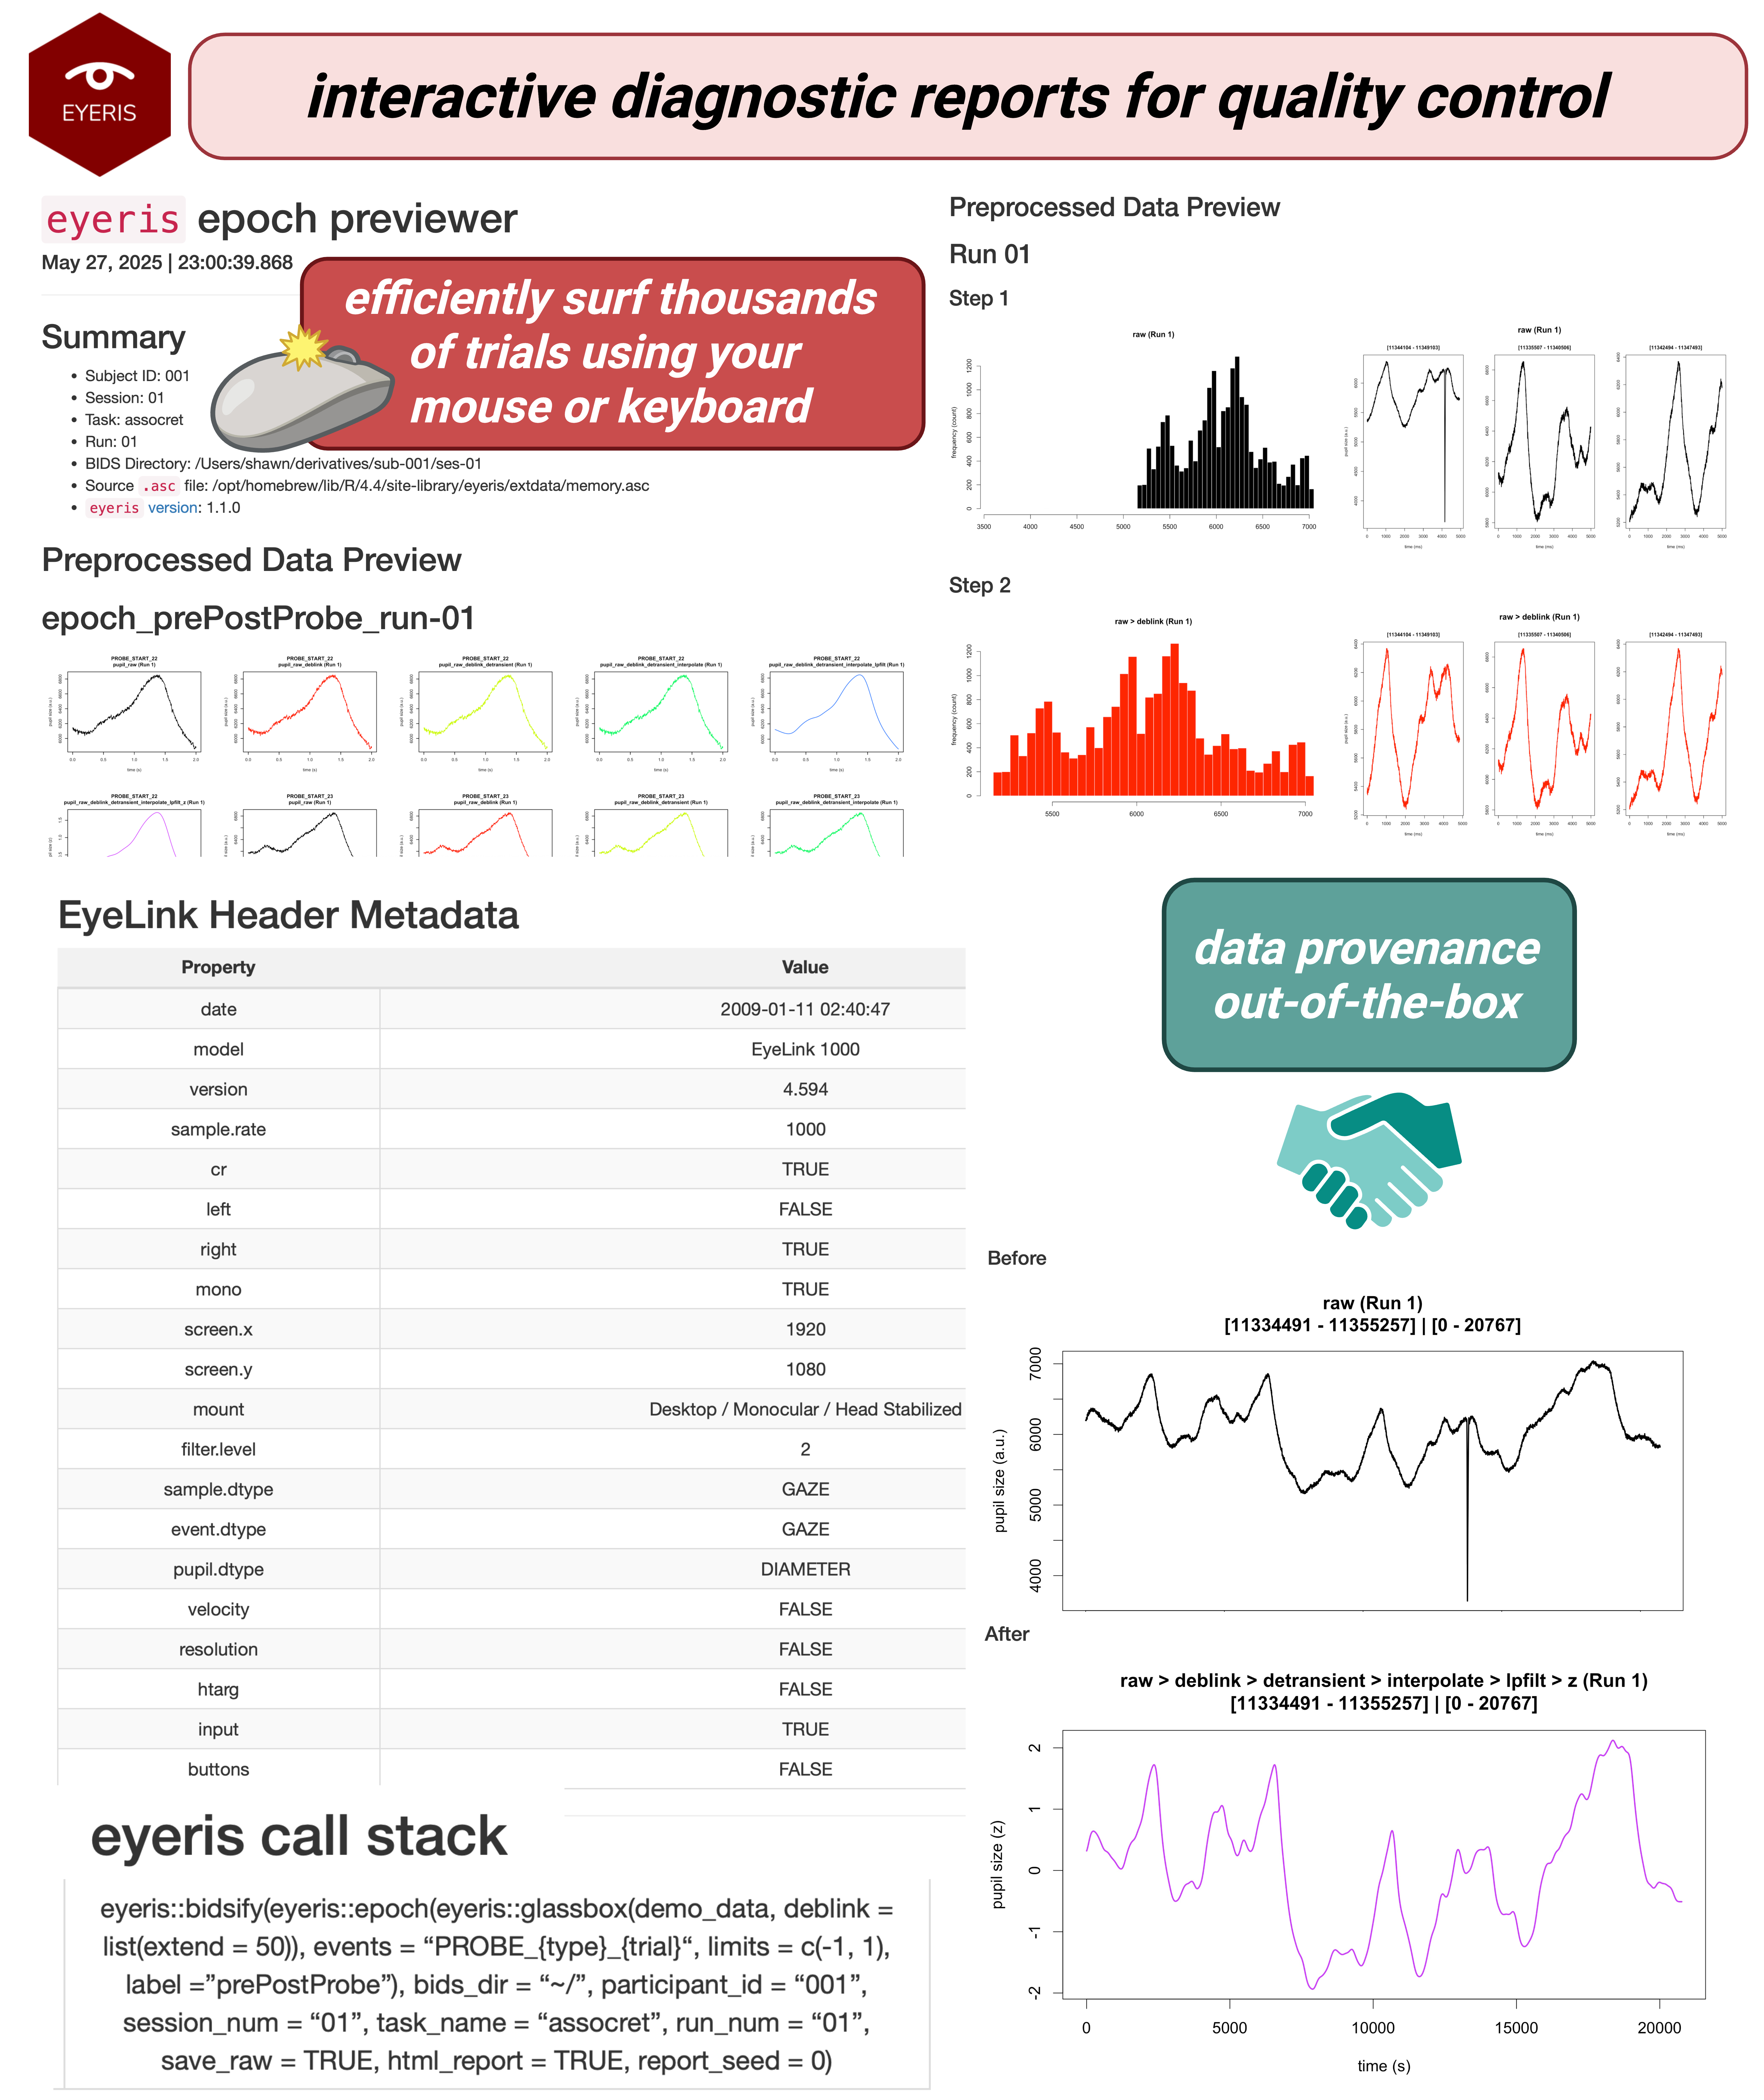
\includegraphics[width=1\linewidth]{figures/eyeris-fig2.jpg}
	\caption[Overview of data and signal processing provenance provided out-of-the-box]{Overview of data and signal processing provenance provided out-of-the-box. eyeris provides automatically generated summary reports with diagnostic plots, recording metadata, and all preprocessing operations/parameters — and the resulting effects of each operation on the pupil time series — for every file/run for every participant. eyeris reports facilitate quality control by enabling surfing through thousands of trials worth of pupil data efficiently and interactively. Furthermore, these reports provide data provenance out-of-the-box and can be shared alongside any publication to support best practices in open science and reproducibility. Created in BioRender \parencite{schwartz2025eyerisreports}. \url{https://BioRender.com/j2h2hzs}.}
	\label{fig:eyeris-fig2}
\end{figure}
\FloatBarrier

\subsubsection{User-friendly pattern matching and metadata parsing make extracting trial level epochs both accurate and effortless.}
Extant solutions for preprocessing pupil data lack intuitive workflows to extract trial-level epochs. For EEG researchers used to functions like pop\_epoch in the MATLAB-based EEGLAB software \parencite{delorme2004eeglab}, the lack of a comparable analogous function can lead to bottlenecks in a researcher’s pupillometry preprocessing workflow. Naturally, it made sense to take inspiration from EEGLAB when designing the epoch() function within eyeris. In particular, extracting trial-level data epochs with eyeris is flexible and offers advanced tooling for the extraction of metadata from event message strings. To illustrate, a researcher may have event message tags that look something like: PROBE\_START\_32\_PIANO, indicating the timestamp for the stimulus probe onset on trial 32 where the stimulus was the piano. While not all event message strings contain as much information as this contrived example (e.g., standard EyeLink trial markers TRIALID 1 often provide helpful trial-number metadata), the additional sources of information in the former example can be leveraged by the researcher as an additional sanity check to ensure accurate linking of pupil data with behavioral and/or neuroimaging data prior to analysis. Unsurprisingly, with more complex event message strings comes more burden on the researcher to devise an accurate and reliable solution to handle their specific event message configuration, likely leading to inefficient one-off solutions for particular datasets. eyeris meets this common demand by providing a carefully crafted regular expression implementation designed to handle a wide variety of generic cases (Box~\ref{box:epoch}).

Conceptually, there are numerous ways that a researcher might want to extract their trial epochs for downstream analysis. In the simplest scenario, the user may be interested in testing a hypothesis about the tonic pupil size in the 1-second period just before the onset of the stimulus. In this case, the user would need to provide the string pattern and fixed start/stop duration of the epoch they would like to extract. For example, c(-1,0) for the 1-second just before the onset of the trial specifies a start/stop time array using the matched event message strings as the reference point (i.e., time=0).

\subsubsection{Interactive visual reports and a BIDS-like data scheme enable intuitive quality control and transparent data reporting.}\label{sec:visual-reports}
To date, most tools for preparing pupillometry data lack suitable features for data quality control up to the individual trial level. While some packages have integrated helpful plotting functions \parencite[e.g.,][]{forbes2020pupillometryr,hershman2019chap,mittner2020pypillometry,tsukahara2020pupillometry}, these approaches only get the user part of the way there, as the onus falls on the user to aggregate such plots in a meaningful way for quality control. Moreover, this significant hurdle could be an arduous task even for researchers with programming experience. We strongly recommend that researchers carefully inspect the data at each stage of the preprocessing pipeline before aggregating trials and/or running inferential statistics, as is common in other human neuroscience data modalities such as EEG with the EEGLAB interactive viewer \parencite{delorme2004eeglab}, M/EEG with MNE-Python \parencite{gramfort2013meg}, fMRI with fMRIPrep \parencite{esteban2019fmriprep}, and structural MRI with MRIQC \parencite{esteban2017mriqc,provins2023quality} visual reports.

Given the lack of generic plug-and-play quality control solutions to date – in addition to the amount of effort required to implement such a solution – we suspect that many published pupillometry studies may not have raw data readily inspected end-to-end before and after preprocessing and running statistics. We therefore provide users with visualization tools of the pupil time series before and after each preprocessing operation for both an entire block/task and every trial-level epoch (i.e., as delineated by event messages/epochs). With this key feature, we hope to lower the barrier required for researchers to visually inspect entire recording sessions for anomalies in an efficient manner, as is necessary to ensure reproducible research results.

For the above reasons, we made visual reporting the default behavior in eyeris (Figure~\ref{fig:eyeris-fig2}). Similar to the goals put forth by the team behind fMRIPrep, we anticipate that automatically generating diagnostic reports per participant will (i) maximize shareability and transparency between researchers, (ii) make data surfing less cumbersome and more efficient and hence increase the probability that thorough data surfing occurs before submitting data to statistical tests, (iii) increase statistical power of future pupillometry investigations by enabling researchers to purge poor data at the trial level without excluding entire runs or participants altogether, and (iv) contribute to best practices in open and reproducible science by recording all preprocessing decisions and settings for any given dataset that makes its way through eyeris by default \parencite{esteban2020analysis,esteban2019fmriprep,poldrack2019computational}.

Importantly, all derived data and reports from the foregoing preprocessing workflows are automatically sorted into a BIDS-like format \parencite{gorgolewski2016brain}, facilitating separation of source (i.e., original or raw) data from derived (i.e., preprocessed, trimmed, epoched, etc.) data, in a directory structure that is intuitive to navigate, automatically organized, and therefore essentially ready to share on an appropriate data sharing outlet/repository like OSF, dryad, and/or GitHub (see Box~\ref{box:bids}).

\subsubsection{Integrated database storage enables scalable and efficient management of large-scale pupillometry datasets.}
As pupillometry research increasingly involves large sample sizes, multi-session designs, and high-throughput cloud computing deployments, traditional CSV-based data management workflows can become unwieldy. For studies with hundreds or thousands of participants – each generating multiple recording files, preprocessing derivatives, epoch extractions, and diagnostic metadata – the resulting proliferation of individual CSV files poses challenges for data organization, storage efficiency, and analytic tractability. Moreover, syncing and transferring thousands of small files across cloud storage systems incurs significant I/O overhead, and loading entire datasets into memory for analysis is often impractical.

To address these scalability challenges, eyeris provides an integrated database storage backend powered by DuckDB \parencite{raasveldt2019duckdb}, a high-performance embedded analytical database engine. When database storage is enabled within the bidsify() function (by setting db\_enabled = TRUE), all preprocessed data – including time series, events, blinks, epochs, epoch summaries, and confounds – are written to a single, self-contained database file (.eyerisdb). This centralized storage approach offers several key advantages over flat-file workflows. First, queries execute at the storage level, allowing researchers to filter, aggregate, and join data across subjects without loading entire datasets into memory. Second, a single database file dramatically reduces I/O costs on cloud platforms compared to syncing thousands of individual files. Third, built-in schema validation maintains data integrity and automatically tracks metadata such as creation timestamps, data types, and relationships between tables. Fourth, researchers can leverage SQL for complex cross-subject filtering and targeted extraction of data subsets, while the eyeris\_db\_collect() wrapper function provides a user-friendly interface that requires no SQL knowledge.

Critically, the database workflow is designed to complement – not replace – the existing BIDS-like file structure described above. Users may choose to generate both CSV files and a database simultaneously, maintaining human-readable outputs alongside the database for transparency, or opt for a database-only workflow to minimize storage and I/O costs in cloud computing environments (e.g., when deploying eyeris on high-performance computing clusters). This flexibility ensures that eyeris can scale from small desktop analyses involving a handful of participants to large-scale, multi-site pupillometry studies with hundreds or thousands of recordings, without requiring researchers to fundamentally change their preprocessing workflow.

For collaborative research and open-science workflows, eyeris also provides tools for distributing large databases in portable formats. The eyeris\_db\_to\_chunked\_files() function enables chunked export of large databases to CSV or Parquet files, processing data incrementally to avoid memory constraints and automatically splitting files that exceed a configurable size threshold. The Parquet format, in particular, offers substantial advantages for archival and sharing: 50–80\% file size reduction compared to CSV, faster read performance, and preserved numeric precision. Together with eyeris\_db\_split\_for\_sharing() and eyeris\_db\_reconstruct\_from\_chunks(), these tools enable seamless data distribution and reconstruction, further supporting the FAIR principles that underpin eyeris.

\subsubsection{Advanced features for developers.}\label{sec:dev-features}
We provide developers the flexibility to extend upon eyeris’ default offerings by writing their own custom pipeline operations that can integrate seamlessly with eyeris primitives (see Box~\ref{box:extensions}).

Under the hood, each preprocessing function in eyeris is a wrapper around a core operation that gets tracked, versioned, and stored using the pipeline\_handler() function. The pipeline\_handler() enables flexible integration of custom data processing functions into the eyeris pipeline. It accepts an eyeris class object, the name of the operation function to apply, a character string suffix for the new column name, and any additional custom parameters. The function returns an updated eyeris object with the new column added to the timeseries data frame and the latest pointer updated to reflect the full history of preprocessing steps (e.g., pupil\_raw → pupil\_raw\_deblink → pupil\_raw\_deblink\_detransient → pupil\_...). Following the eyeris protocol ensures that all operations follow a predictable structure and that new pupil data columns based on previous operations in the chain are dynamically constructed within the core time series data frame. Custom pipeline steps must conform to this protocol for maximum compatibility with the downstream functions we provide.

To demonstrate the flexibility of eyeris for developers, we walk through building a custom extension below. Please note that in the example that follows, we are not recommending that one performs this particular statistical transformation on their pupil data; rather, this is purely for demonstration purposes. Suppose you want to write a new eyeris extension function called winsorize() to apply winsorization to extreme pupil values. First, you write the core operation function, which should accept a data frame x, a string prev\_op (the name of the previous pupil column), and any custom parameters. Second, you create a wrapper using the pipeline\_handler() function, which enables your function to automatically: (a) track your function within the eyeris list object’s params field, (b) append a new column to each block within the timeseries list of data frames, and (c) update the object’s latest pointer. To ensure compatibility with eyeris, we impose the following requirements for any custom extension functions: (1) the first argument is always the eyeris class object; (2) the second is the name of the core operation function; (3) the third is the internal label you want eyeris to refer to (i.e., the one for the column name, plots, etc.); and (4) the fourth position onward are the custom parameters you defined in the core operation function. See Appendix~\ref{app:custom-extensions} for all source code for this demo. More information about customizing eyeris can be found in the online package documentation.

\section{Conclusions}
The bells and whistles detailed throughout this manuscript and the documentation website for the eyeris R package aim to standardize the way pupillometry data are preprocessed and used in downstream analysis. To this end, we designed the architecture underlying eyeris to support the building of a robust suite of pupillometry tools analogous to the current offerings for fMRI analysts with fMRIPrep \parencite{esteban2020analysis,esteban2019fmriprep}. At its core, eyeris enables standardized and flexible preprocessing of the pupil assay.

Moreover, eyeris was designed with FAIR principles in mind. To fulfill this promise, eyeris uses a built-in protocol to carry out and manage the record keeping of the entire preprocessing pipeline on a raw dataset (see Figure~\ref{fig:eyeris-fig1}). This protocol is more or less a ``grammar'', where each operation is a ``verb'' that can be chained one after the other \parencite[see Box~\ref{box:extensions}, which draws inspiration from familiar tidyverse ``pipe'' workflows;][]{wickham2019welcome}. This approach allows us to take advantage of syntactic sugar such that one could take a raw pupillometry dataset and within seconds obtain (i) a step-by-step record of all preprocessing steps (and parameters used), (ii) how each step sequentially impacted the raw signal, (iii) default diagnostic reports that organize relevant preprocessing metadata for any particular dataset passed through eyeris, and (iv) an intuitive gallery viewing functionality for efficiently scrolling through hundreds-to-thousands of raw data epochs for quality control prior to running inferential statistics (Figure~\ref{fig:eyeris-fig2}).

Additionally, eyeris provides integrated database storage powered by DuckDB, enabling researchers to manage and query preprocessed pupillometry data from large-scale studies – involving hundreds or thousands of participants – within a single, self-contained database file. This database backend, combined with chunked export tools for portable data sharing in CSV and Parquet formats, ensures that eyeris can scale from small desktop analyses to cloud-deployed, multi-site studies without compromising on the transparency, reproducibility, or accessibility of the preprocessing workflow.

An important current limitation of eyeris is that it supports only SR Research EyeLink .asc files as input. While EyeLink systems remain widely used in cognitive pupillometry, this restriction excludes researchers using alternative eye-tracking hardware (e.g., Tobii, Pupil Labs, GazePoint). Extending eyeris to support additional systems involves more than implementing new file loaders: different eye trackers produce qualitatively different artifact profiles. For example, EyeLink systems tend to produce characteristic sharp downward spikes flanking blinks due to partial pupil occlusion by the eyelid, whereas video-based trackers may exhibit different artifact morphologies that could require adjusted detection parameters or different rejection strategies entirely. The modular architecture of eyeris — in particular, the pipeline\_handler() system and the separation of file loading from downstream preprocessing — was designed to accommodate such extensions. The load\_asc() function can serve as a template for future hardware-specific loaders (e.g., load\_tobii(), load\_csv()), and tracker-specific preprocessing steps can be integrated as custom extensions without modifying the core framework. Moreover, we are currently developing a generic CSV-based ingestion pathway that will allow users to provide a column mapping specification for arbitrary tabular eye-tracking data, and we welcome community contributions of additional loaders via the project's GitHub repository (see Code Availability). Despite this input limitation, the signal processing principles underlying each preprocessing step — blink artifact removal, transient detection, interpolation, filtering, and normalization — are generally applicable across eye-tracking systems, even as specific default parameters may require re-tuning for different hardware.

We also note that eyeris is intentionally scoped as a preprocessing framework: it transforms raw tracker files into cleaned, epoched, and export-ready data, but does not itself implement statistical analysis or group-level visualization. However, the transition from preprocessing to analysis is straightforward. The epoched output from eyeris is a tidy data frame (one row per sample, with columns for participant, trial, condition metadata, time, and preprocessed pupil size) that is directly amenable to analysis with linear mixed-effects models (e.g., via lme4 or brms in R), enabling researchers to analyze entire multi-participant datasets simultaneously without first computing participant-level averages. The DuckDB database backend further supports this workflow: eyeris\_db\_collect() can aggregate preprocessed data across all participants into a single table for group-level analysis and visualization with standard tidyverse tools. For detailed guidance on the statistical analysis stage of cognitive pupillometry, we refer users to \textcite{mathot2023methods}, whose analysis recommendations integrate naturally with the tidy output format produced by eyeris. A complete end-to-end tutorial from raw data through group-level analysis is available in the package documentation (\url{https://eyeris.shawnschwartz.com}).

To this end, our hope is that enabling access to intuitive, interactive visual inspection tools to efficiently assess trial/epoch-level data quality – combined with scalable data management infrastructure – at scale, will support researchers in their efforts to perform reproducible and rigorous pupillometry research in a more accessible manner than is afforded by extant offerings.